\documentclass[a4paper,12pt]{article}
\usepackage[utf8]{inputenc}      % Codificación UTF-8 para caracteres en español
\usepackage[T1]{fontenc}         % Buena salida de fuentes
\usepackage[spanish]{babel}      % Traducción de elementos automáticos al español
\usepackage{lmodern}             % Fuente mejorada
\usepackage[hidelinks]{hyperref} % Para enlaces, [hidelinks] elimina el reborde azul del .pdf
\usepackage{graphicx}            % Para incluir imágenes (PNG)
\usepackage{float}               % Para anclar las imagenes a una posicion fija
\usepackage{bytefield}           % Para dibujar diagramas PDU
\usepackage{geometry}            % Para ajustar márgenes
\usepackage{placeins}

\geometry{left=2.5cm, right=2.5cm, top=3cm, bottom=3cm}

\title{El protocolo IPv6}
\author{Martín Moloeznik, Nicolás Paz Reyes\\[0.5em]
Repositorio: \url{https://github.com/tu_usuario/tu_repositorio}}
\date{\today}

\begin{document}

% Carátula
\begin{titlepage}
  \centering
  \vspace*{2cm}
  {\large \textbf{El protocolo IPv6}}\\[1.5cm]
  
  {\large Integrantes:}\\
   \bigskip
  {\large Martín Moloeznik, Nicolás Paz Reyes} \\[0.5cm]
  {\large {martinmoloeznik@gmail.com}, {rubenpaz2105@gmail.com}} \\[0.5cm]
  \bigskip
  {\large Repositorio: \url{https://github.com/N1C0-P4Z/Protocolo-IPv6}}\\[1cm]
  
  \vfill
  {\large \today}
\end{titlepage}

% Índice (opcional)
\tableofcontents
\newpage

% Sección de Introducción
\section*{Introducción}
\setcounter{section}{0}
El protocolo IPv6 fue desarrollado para reemplazar a IPv4 debido a la necesidad de una mayor cantidad de direcciones IP en el mundo. Dentro de IPv6 existen mecanismos esenciales para la configuración de direcciones y la comunicación entre dispositivos, entre los cuales se destacan SLAAC, EUI-64 y el protocolo Neighbor Discovery (NDP).

% Sección 1: Escenarios y Configuraciones
\section{IPv6 SLAAC and EUI-64 Basics}
\subsection{Configuración del Router en IPv6}

%ACA VA UNA IMAGENNNN QUE NICO BORRO PARA NO GENERAL PROBLEMAS

Mediante los siguientes comandos configuramos la Link Local Address del router a fe80::1 y la GUA a 2001:db8:acad:1::1/64.\\

\noindent Router\#enable\\
Router\#configure terminal\\
Router(config)\#ipv6 unicast-routing\\
Router(config)\#interface g0/0\\
Router(config-if)\#ipv6 enable\\
Router(config-if)\#ipv6 address fe80::1 link-local\\
Router(config-if)\#ipv6 address 2001:db8:acad:1::1/64\\
Router(config-if)\#no shutdown\\

\subsection{Explicacion algoritmo EUI-64}
   La PC se autoconfigura su Link Local Addres siguiendo los pasos a continuacion:

\bigskip
\begin{bytefield}[boxformatting={\centering\itshape},bitwidth = 1.1em]{32}
  \begin{rightwordgroup}{Algoritmo \\ EUI-64}

    \bitbox{16}{48 bit MAC} & \bitbox{16}{00-E0-F9-98-8A-07}\\
    \bitbox{16}{Separa al medio} & \bitbox{16}{00-E0-F9 \hspace{0.45cm} | \hspace{0.45cm} 98-8A-07}\\
    \bitbox{16}{Insertar FF-FE} & \bitbox{16}{00-E0-F9 \textbf{FF-FE} 98-8A-07}\\
    \bitbox{16}{Primeros dos hexa a binario} & \bitbox{16}{0000-0000-E0-F9  \textbf{FF-FE} 98-8A-07}\\
    \bitbox{16}{Se invierte el septimo bit} & \bitbox{16}{0000-00\textbf{1}0-E0-F9  \textbf{FF-FE} 98-8A-07}\\
    \bitbox{16}{64 bits host interface ID} & \bitbox{16}{\textbf{02}-E0-F9-\textbf{FF-FE}-98-8A-07}\\
    \bitbox{16}{Link Local Address} & \bitbox{16}{FE80::\textbf{2E0:F9FF:FE98:8A07}}
  \end{rightwordgroup}
\end{bytefield}
\subsection{Router Solicitation}
\bigskip
Luego entramos al modo simulación y cambiamos la configuración ipv6 de la pc de static a  auto-config, inmediatamente, la pc envía un mensaje de router solicitation. Donde la ip de origen es la LLA de la pc que se autoconfiguró mediante EUI-64 y la ip destino es la ALL routers multicast address.

\bigskip

\begin{bytefield}[boxformatting={\centering\itshape},bitwidth = 1.1em]{32}
  \bitheader{0,4,12,32} \\
  \bitbox{4}{Ver:6} & \bitbox{8}{TRFC} & \bitbox{20}{FLOW LABEL}\\
  \bitbox{16}{PL:12} & \bitbox{8}{NEXT:0x3a} & \bitbox{8}{HOP LIMIT:255}\\ 
  \begin{rightwordgroup}{Link Local\\ Address}
    \wordbox{2}{SRC IP:FE80::2E0:F9FF:FE98:8A07}
  \end{rightwordgroup}\\
  \begin{rightwordgroup}{All Routers\\ Multicast \\address}
    \wordbox{2}{DEST IP:FF02::2}
  \end{rightwordgroup}
\end{bytefield}

\subsection{Router Advertisement}

\bigskip

La PC aprende que se esta usando IPv6 y a la LLA del router que usará como gateway.
\bigskip

\begin{bytefield}[boxformatting={\centering\itshape},bitwidth = 1.1em]{32}
  \bitheader{0,8,16} \\
  \bitbox{4}{VER:6} & \bitbox{8}{TRFC} & \bitbox{20}{FLOW LABEL} \\
  \bitbox{16}{PL:60} & \bitbox{8}{NEXT:0x3a} & \bitbox{8}{HOP LIMIT:255} \\
  \wordbox{2}{SRC IP: FE80::1} \\
  \wordbox{2}{DST IP: FF02::1}
\end{bytefield}

\bigskip
El router responde con el siguiente mensaje de Router Advertisement:

\bigskip

\begin{bytefield}[boxformatting={\centering\itshape},bitwidth = 1.1em]{32}
  \bitheader{0,8,16} \\
  \bitbox{8}{TYPE: 0x86} & \bitbox{8}{CODE: 0x00} & \bitbox{16}{CHECKSUM: 0x0000} \\
  \bitbox{8}{Hop Limit: 0x40} & \bitbox{8}{RESERVED} & \bitbox{16}{Router Lifetime: 0x0708} \\
  \bitbox{32}{Reachable Time: 0x00000000} \\
  \bitbox{32}{Retrans Timer: 0x00000000}
\end{bytefield}

\bigskip
\subsection*{Prefix Option}
\begin{bytefield}[boxformatting={\centering\itshape},bitwidth = 1.1em]{32}
  \bitheader{0,8,16} \\
  \bitbox{8}{TYPE: 0x03} & \bitbox{8}{LENGTH: 0x04} & \bitbox{8}{PREFIX LEN: 64} & \bitbox{8}{RESERVED1} \\
  \bitbox{32}{VALID LIFETIME: 2592000} \\
  \bitbox{32}{PREFERRED LIFETIME: 604800} \\
  \bitbox{32}{RESERVED2} \\
  \bitbox{32}{PREFIX: 2001:DB8:ACAD:1::}
\end{bytefield}

\bigskip
Aquí la PC aprende el prefijo de red, su tamaño, el tipo y por cuanto tiempo es valida esta informacion. De esta forma, la PC se autoconfigura su IPv6 Global Unicast Address, ya que tiene todos los elementos necesarios. Usará como interface ID lo que ya aprendio usando el algoritmo EUI-64.
\bigskip

\begin{bytefield}[boxformatting={\centering\itshape},bitwidth = 1.1em]{32}
  \bitheader{0,8,16} \\
  \bitbox{8}{TYPE: 0x01} & \bitbox{8}{LENGTH: 0x01} & \bitbox{16}{} \\
  \wordbox{2}{LINK LAYER ADDRESS: 0060.3E5A.5801}
\end{bytefield}

\bigskip
En este mensaje, la PC aprende la Link Layer Address del Router.

% Sección 2: Escenario 2: Neighbor Discovery
\section{Neighbor Discovery}

%ACA VA UNA FOTO DEL ESCENARIO

Configuramos las IPs de las PCs y el Router con los comandos que vimos en el apartado anterior. Luego nos aseguramos que el R0 no tenga información de sus vecinos con
\bigskip

\noindent R0\#show ipv6 neighbors\\

\subsection{Local Delivery}

Realizaremos un ping desde la consola de P0 a P1 en el modo simulación, filtrando los mensajes ICMPv6 y NDP para visualizarlos en la \textit{Event List} 

\subsubsection{Mensaje NDP}

En el tercer evento vemos que la PC0 envia un PDU NDP al Switch0. Este PDU va a ser de tipo 135 Neighbor Solicitation, con el objetivo de descubrir la dirección MAC de los otros dispositivos en la misma red local. El mensaje de Neighbor Solicitation se ve representado de la siguiente manera:

\bigskip

\begin{bytefield}[boxformatting={\centering\itshape},bitwidth = 1.1em]{32}
  \bitheader{0,8,16} \\
  \bitbox{8}{TYPE: 0x87} & \bitbox{8}{CODE: 0x00} & \bitbox{16}{CHECKSUM} \\
  \bitbox{1}{R} & \bitbox{1}{S} & \bitbox{1}{O} & \bitbox{29}{Reserved} \\
  \bitbox{32}{Target Address: 2001:DB8:ACAD:1::B}
\end{bytefield}

\bigskip

En TYPE se muestra en hexadecimal 0x87, que en decimal es 135, confirmando que el mensaje es de tipo Neighbor Solicitation. En el 4to y 5to evento vemos que el Switch hizo forward del NDP a la PC1 y al Router.

\bigskip

La respuesta va a ser una PDU NDP de tipo Neighbor Advertisement, es decir Type 136(0x87 en hexadecimal).

\bigskip

\begin{bytefield}[boxformatting={\centering\itshape},bitwidth = 1.1em]{32}
  \bitheader{0,8,16} \\
  \bitbox{8}{TYPE: 0x88} & \bitbox{8}{CODE: 0x00} & \bitbox{16}{CHECKSUM} \\
  \bitbox{1}{R} & \bitbox{1}{S} & \bitbox{1}{O} & \bitbox{29}{Reserved} \\
  \bitbox{32}{Target Address: 2001:DB8:ACAD:1::B}
\end{bytefield}

\bigskip

Esta respuesta llega al Switch, el cual nuevamente fordwardea por todas sus interfaces, menos por la que recibió el mensaje. La PC1 lo descarta y la PC0 lo acepta.

\bigskip

De esta manera mostramos cómo funcionan los mensajes de Neighbor Solicitation y Neighbor Advertisement. 

\bigskip
\subsubsection{Mensaje ICMPv6}

En el primer evento, seleccionamos el mensaje ICMPv6 en la PC0, para analizar la PDU.

%ACA VA UNA FOTOOOO seria el P2

Observamos que es un mensaje ICMPv6 de TYPE 0x80, es decir 128 en decimal, lo que corresponde a un mensaje ECHO REQUEST, que cuenta con la siguiente estructura:

\bigskip

\begin{bytefield}[boxformatting={\centering\itshape},bitwidth = 1.1em]{32}
  \bitheader{0,8,16} \\
  \bitbox{8}{TYPE: 0x80} & \bitbox{8}{CODE: 0x00} & \bitbox{16}{CHECKSUM: 0x0000} \\
  \bitbox{16}{IDENTIFIER: 2} & \bitbox{16}{SEQUENCE NUMBER: 1}
\end{bytefield}

\bigskip

También podemos observar que la sección Out Layers del OSI Model se resuelve en la layer 3.

\bigskip

Luego presionamos en Next Layer y nos aparece una salida con lo sucedido en la Layer 2.

\bigskip

Nos explica que el next hop es una dirección unicast, por lo que el proceso de Neighbor Discovery la busca en la neighbor table. Luego ve que el next hop no se encuentra en la tabla, por lo que el protocolo NDP envía una neighbor solicitation, comenzando el proceso visto en el apartado anterior.

\bigskip

\subsubsection{Cómo recibe el Router los mensajes del protocolo NPD?}

Seleccionamos el próximo evento, el mensaje NDP en la PC0 y observamos que la dirección de destino cambió por una dirección multicast de enlace local (FF02::) que utiliza el proceso de Neighbor Discovery. 

\bigskip

En la layer 2 vemos que tenemos la dirección MAC de origen de la PC0 y la dirección MAC de destino que es 3333.FF00.000B, que es una dirección de multidifusión. Lo que tiene de particular esta dirección es que pertenece al rango de direcciones de multidifusión de la layer 2, asignadas a IPv6. Los ultimo 32 bits de la dirección MAC coinciden con los últimos 32 bits de la dirección IPv6 de multidifusión.

\bigskip

Esto permite que el descubrimientos de vecinos sea mucho mas eficiente en redes IPv6.

\bigskip

\subsubsection{Próximo evento en el Switch 0}

Seleccionamos el próximo evento que ocurre en el Switch 0, y observamos que no ocurren cambios en la entrada y salida en la capa 2. Esto ocurre ya que el switch no altera o cambia nada en las tramas, solo las reenvía por todos sus puertos, excepto por el de entrada.

\bigskip

\subsubsection{Información sobre el primer evento en PC1}

\begin{itemize}
    \item Ethernet Destination Address: \textit{3333.FF00.000B}
    \item Ethernet Source Address: \textit{0090.0C5B.E7DC}
    \item IPv6 Source Address: \textit{2001:DB8:ACAD:1::B}
    \item IPv6 Destination Address: \textit{FF02::1:FF00:B}
\end{itemize}

\bigskip

\subsubsection{Falta de Información en Out Layers}

Al seleccionar el primer evento en el Router 0, en el que el router recibe el mensaje NDP forwardeado desde el Switch, observamos que en las Out Layers no hay información porque la dirección IP destino del mensaje NDP es la de la PC1, y no la del Router. El Router entiende que el mensaje no es para él y la descarta.

\bigskip

\subsubsection{Proximo paquete ICMPv6}

Seleccionamos el próximo evento ICMPv6 de la PC0 y observamos que efectivamente tiene toda la información para comunicarse con la PC1.

\bigskip

%ACA VA UNA FOTOOOOOOOOO

Efectivamente la PC0 tiene la dirección de IP destino y la dirección MAC de destino de la PC1, por lo que ahora la comunicación entre PCs debería ser exitosa.

\bigskip

\subsubsection{Ultimo evento de la lista}

En el último evento de la lista, que es un mensaje ICMPv6 de PC0, vemos que es un ECHO MESSAGE TYPE 129, es decir, \textit{Echo Reply}.

\bigskip

\subsubsection{Resetear la simulación}

Reseteamos la simulación y volvemos a hacer un ping entre la PC0 y la PC1 mediante comandos, y observamos la ausencia del proceso Neighbor Discovery, ya que la PC0 ya conoce la MAC de la PC1 gracias al proceso realizado anteriormente.

\bigskip

%ACA VA UNA FOTOOOOOOOOOOOOOOOOOO

Con esta información, la PC0 puede hacer pings a la PC1 cuantas veces quiera. Por esto sólo observamos los eventos ICMPv6 que van del PC0 al Switch, del Switch a la PC1 y las respuestas correspondientes. 

\bigskip




%aca martoooooo!!!! no tocar que me te cojo.
\subsection{Non Local Delivery}

\subsubsection{Configuracion el escenario}
Para analizar el proceso en redes remotas, primero borraremos la informacion sobre neighbors en el Router 0 mediante el comando clear ipv6 neighbors y reseteamos la información.\\
\subsubsection{Comienzo del escenario}
Realizaremos un ping desde la PC0 a la PC2 que tiene la IP 2001:DB8:ACAD:2: :A/64, en el modo simulación para poder ver y analizar la lista de eventos.\\
\subsubsection{Primer Evento en PC0}
Al observar el primer evento en la PC0, que se trata de un mensaje ICMPv6, vemos que no hay información en la capa 2, ya que la PC0 todavía no sabe la MAC address de la PC2.\\
\begin{figure}[h]
    \centering
    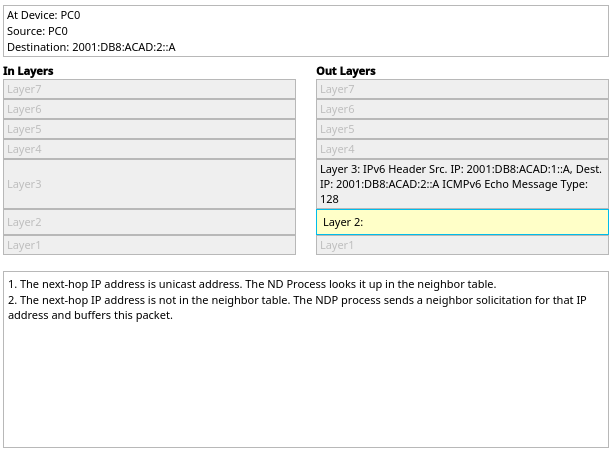
\includegraphics[width=0.7\textwidth]{imagenes/1.png}
    \caption{Primer ICMPv6 Pc0}
\end{figure}\\
\subsubsection{Segundo Evento en la PC0}
Al observar el primer mensaje NDP en la PC0, vemos que es un Neighbor Solicitation, ya que es de tipo 0x87(135 en decimal) al igual que anteriormente en el Local Delivery. La dirección IPv6 de origen es la Link Local Address de la PC0, la cual es FE80::290:2BFF:FE89:2D86.\\
\begin{figure}[h]
    \centering
    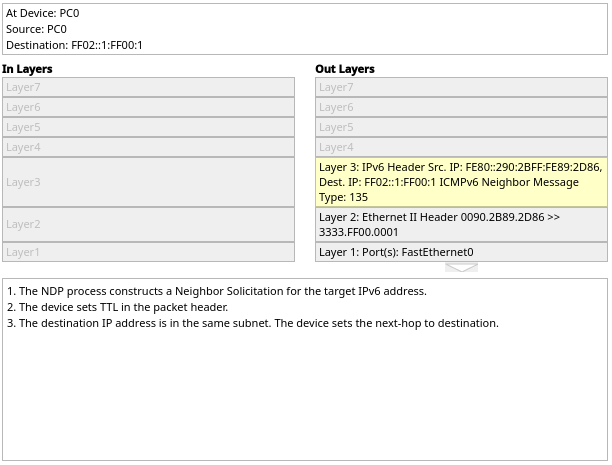
\includegraphics[width=0.7\textwidth]{imagenes/2.png}
    \caption{Primer NDP Pc0}
\end{figure}\\
\FloatBarrier
\subsubsection{Próximo Evento ICMPv6 en la PC0}
Buscamos el siguiente mensaje ICMPv6 que sale de la PC0. Comprobamos que ahora si tiene información en la capa 2. La MAC de origen es la MAC address de la PC0 y se utiliza la MAC address de la interfaz g0/0 del router como MAC de destino. Esto se debe a que la única forma de acceder a la PC2, desde la PC0, es utilizando el Router.\\
\begin{figure}[h]
    \centering
    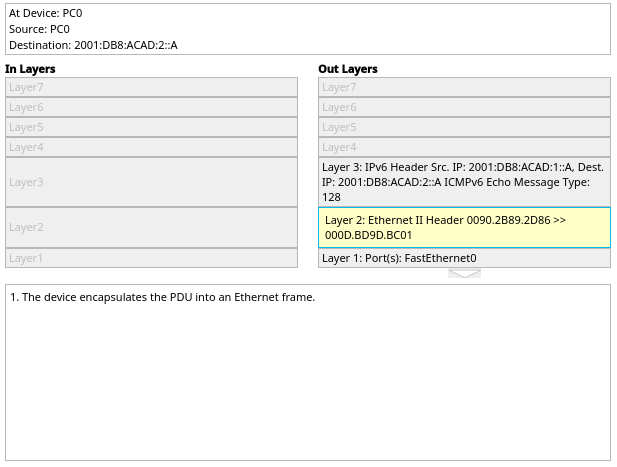
\includegraphics[width=0.7\textwidth]{imagenes/3.png}
    \caption{Siguiente ICMPv6 Pc0}
\end{figure}\\
\FloatBarrier
\subsubsection{Primer evento ICMPv6 en R0}
Observamos el primer evento ICMPv6 en el  Router 0 y comprobamos que la información de la capa 2 está vacía. Esto se debe a que el Router no conoce la MAC address de la PC2, ya que borramos la información de vecinos del Router, por lo que comenzará otro proceso NDP para descubrir la direccion desconocida. \\
\begin{figure}[h]
    \centering
    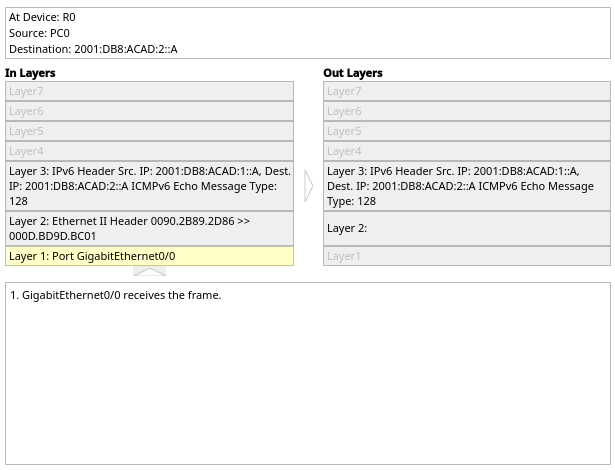
\includegraphics[width=0.7\textwidth]{imagenes/4.png}
    \caption{ICMPv6 R0}
\end{figure}\\

\FloatBarrier

\subsubsection{Evento ICMPv6 en la PC2}
Observamos el próximo evento ICMPv6 en la PC2 y volvemos a ver que la capa 2 está vacía. Esto se debe a que la PC2 no conoce la MAC address para comunicarse con la PC0, por lo que comienza un proceso de NDP.\\
\begin{figure}[h]
    \centering
    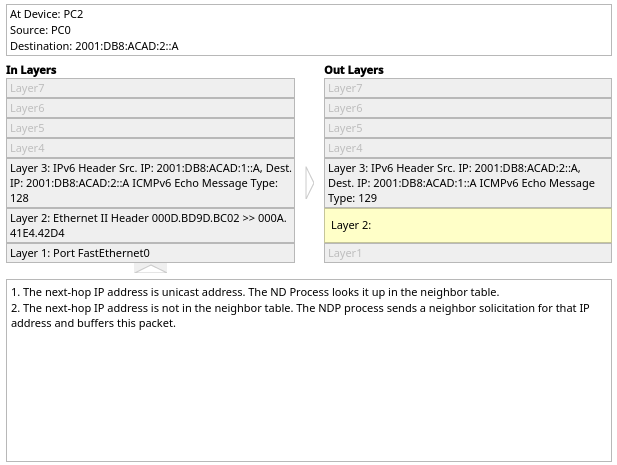
\includegraphics[width=0.7\textwidth]{imagenes/5.png}
    \caption{ICMPv6 Pc2}
\end{figure}\\

\FloatBarrier
\subsubsection{Ultimos eventos ICMPv6}
Al ir al ultimo conjunto de eventos ICMPv6, luego de haber finalizado todos los procesos de NDP, la PC2 ya conoce la MAC address del Router y a su vez, el Router conoce la MAC address de la PC0, por lo que la PC2 puede enviar mensajes de respuesta a la PC0 sin necesidad de ningun mensaje NDP.\\
\subsubsection{Reinicio de simulación}
Esto lo podemos confirmar al reiniciar la simulación volver a hacer ping de la Pc0 a la Pc2 y notamos que no hubo ningún evento NDP. \\
\begin{figure}[h]
    \centering
    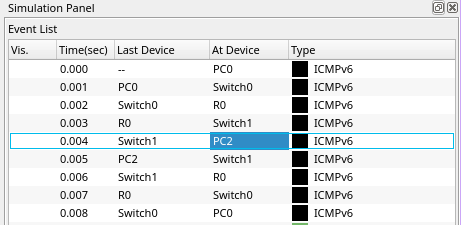
\includegraphics[width=0.7\textwidth]{imagenes/6.png}
    \caption{Ningun NDP}
\end{figure}\\
\FloatBarrier
Al observar el mensaje seleccionado, vemos que en la capa 2 la direccion MAC de destino es la dirección MAC de la interface G0/1 del Router, ya que este es el encargado de relacionar la red de la PC2 con la PC0.
\begin{figure}[h]
    \centering
    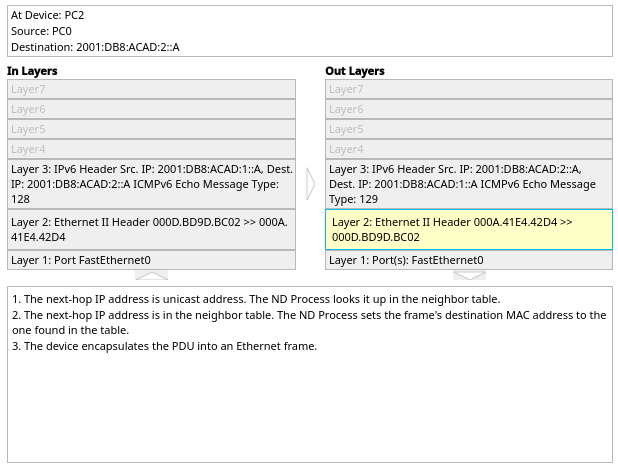
\includegraphics[width=0.7\textwidth]{imagenes/7.png}
    \caption{ICMPv6 Pc2}
\end{figure}\\
\FloatBarrier
\subsubsection{Modo Realtime}
Ingresamos al modo realtime ejecutamos el comando show ipv6 neighbors y vemos la siguiente tabla:\\

\bigskip
\begin{bytefield}[boxformatting={\centering\itshape},bitwidth = 1.1em]{32}
  \bitheader{0,8,16} \\
  \bitbox{16}{IPv6 Address} & \bitbox{4}{Age} & \bitbox{8}{Link-layer Addr} & \bitbox{4}{State} & \bitbox{4}{Interface} \\
  \bitbox{16}{2001:DB8:ACAD:1::A} & \bitbox{4}{0} & \bitbox{8}{0090.2B89.2D86} & \bitbox{4}{REACH} & \bitbox{4}{Gig0/0} \\
  \bitbox{16}{2001:DB8:ACAD:2::A} & \bitbox{4}{0} & \bitbox{8}{000A.41E4.42D4} & \bitbox{4}{REACH} & \bitbox{4}{Gig0/1} \\
  \bitbox{16}{FE80::20A:41FF:FEE4:42D4 } & \bitbox{4}{0} & \bitbox{8}{000A.41E4.42D4} & \bitbox{4}{REACH} & \bitbox{4}{Gig0/1} \\
  \bitbox{16}{FE80::290:2BFF:FE89:2D86} & \bitbox{4}{0} & \bitbox{8}{0090.2B89.2D86} & \bitbox{4}{REACH} & \bitbox{4}{Gig0/0} \\
\end{bytefield}\\
Aquí vemos 4 direcciones, 2 Global Unicast Address (GUA) y 2 Link - Local Address(LLA) que corresponden a las PC0 y PC2. No vemos ninguna entrada que corresponda a la PC1 ya que no la utilizamos hasta este punto.\\
\subsubsection{Ping de R0 a la Pc1}
Realizamos un ping a la PC1 desde el Router y volvemos a ejecutar el comando show ipv6 neighbors:\\

\begin{bytefield}[boxformatting={\centering\itshape},bitwidth = 1.1em]{32}
    \bitheader{0,8,16} \\
    \bitbox{16}{IPv6 Address} & \bitbox{4}{Age} & \bitbox{8}{Link-layer Addr} & \bitbox{4}{State} & \bitbox{4}{Interface} \\
    \bitbox{16}{2001:DB8:ACAD:1::A} & \bitbox{4}{28} & \bitbox{8}{0090.2B89.2D86} & \bitbox{4}{REACH} & \bitbox{4}{Gig0/0} \\
    \bitbox{16}{2001:DB8:ACAD:2::B} & \bitbox{4}{0} & \bitbox{8}{000A.41E4.42D4} & \bitbox{4}{REACH} & \bitbox{4}{Gig0/1} \\
    \bitbox{16}{2001:DB8:ACAD:2::A} & \bitbox{4}{28} & \bitbox{8}{000A.41E4.42D4} & \bitbox{4}{REACH} & \bitbox{4}{Gig0/1} \\
    \bitbox{16}{FE80::20A:41FF:FEE4:42D4 } & \bitbox{4}{28} & \bitbox{8}{000A.41E4.42D4} & \bitbox{4}{REACH} & \bitbox{4}{Gig0/1} \\
    \bitbox{16}{FE80::290:2BFF:FE89:2D86} & \bitbox{4}{28} & \bitbox{8}{0090.2B89.2D86} & \bitbox{4}{REACH} & \bitbox{4}{Gig0/0} \\
\end{bytefield}\\
Vemos una nueva dirección correspondiente a la GUA de la PC1, ya que luego del ping hubo interacción con el router y este aprendió su dirección. IPv6.\\
% Sección de Conclusiones
\section{Conclusiones}
Aquí se sintetizan los resultados obtenidos y se discuten las ventajas y desventajas de la autoconfiguración en IPv6, así como el impacto del proceso de Neighbor Discovery en el rendimiento de la red.

% Sección de Referencias
\section{Referencias}
Para la elaboracion de este informe utilizamos el contenido de los siguientes videos. 
\begin{itemize}
  \item \textbf{Video 1:} “IPv6 SLAAC and EUI-64 Basics in Packet Tracer”, Dan Alberghetti, 2019, at \url{https:
  //www.youtube.com/watch?v=yMK1NVHksDE}.
  \item \textbf{Video 2:} “IPv6 NDP and ICMPv6 using Packet Tracer”, Dan Alberghetti, 2020, at \url{https://www.
  youtube.com/watch?v=y2GpG9aOIFI}
  \item \textbf{Video 3:} “Detección de vecinos IPv6 (Packet Tracer Lab 9.3.4)”, RedesNetw channel, 2022, at \url{https://www.youtube.com/watch?v=ZBVXbgF39gw}
+\end{itemize}

\end{document}
